\section{Component Interfaces}
In these diagrams are shown the main methods offered to the registered users by the interfaces of the components.

\begin{itemize}
    \item  The interface \underline{UserMobileServices} provides all the methods that Users will call to manage their requests, data visualization, emergency services and services related to the run enrollment and the run organization.
    \item The interface \underline{ThirdPartyWebServices} extends the interfaces of the Third Party Web Services subsystem. These interfaces provide all the methods relative to the request of data of individual User or group of Users and also relative to the visualization of the already accessible data.
   \end{itemize}

\begin{figure}[H]

    \centering
    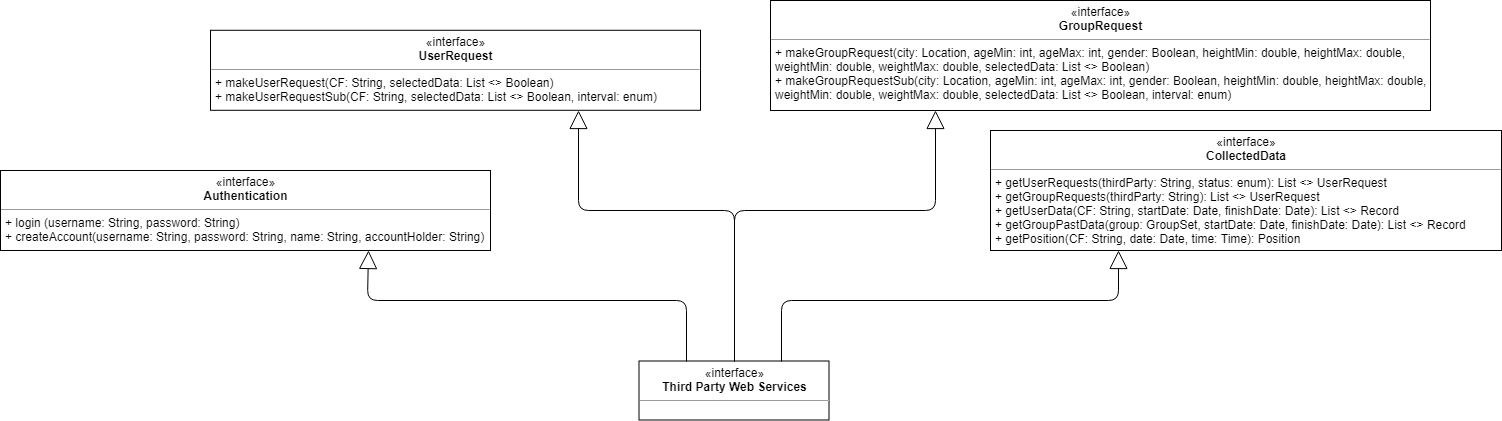
\includegraphics[scale=0.32]{./Pictures/compInterfDiagThirdPDD.png}
   
\end{figure}

\begin{figure}[H]

    \centering
    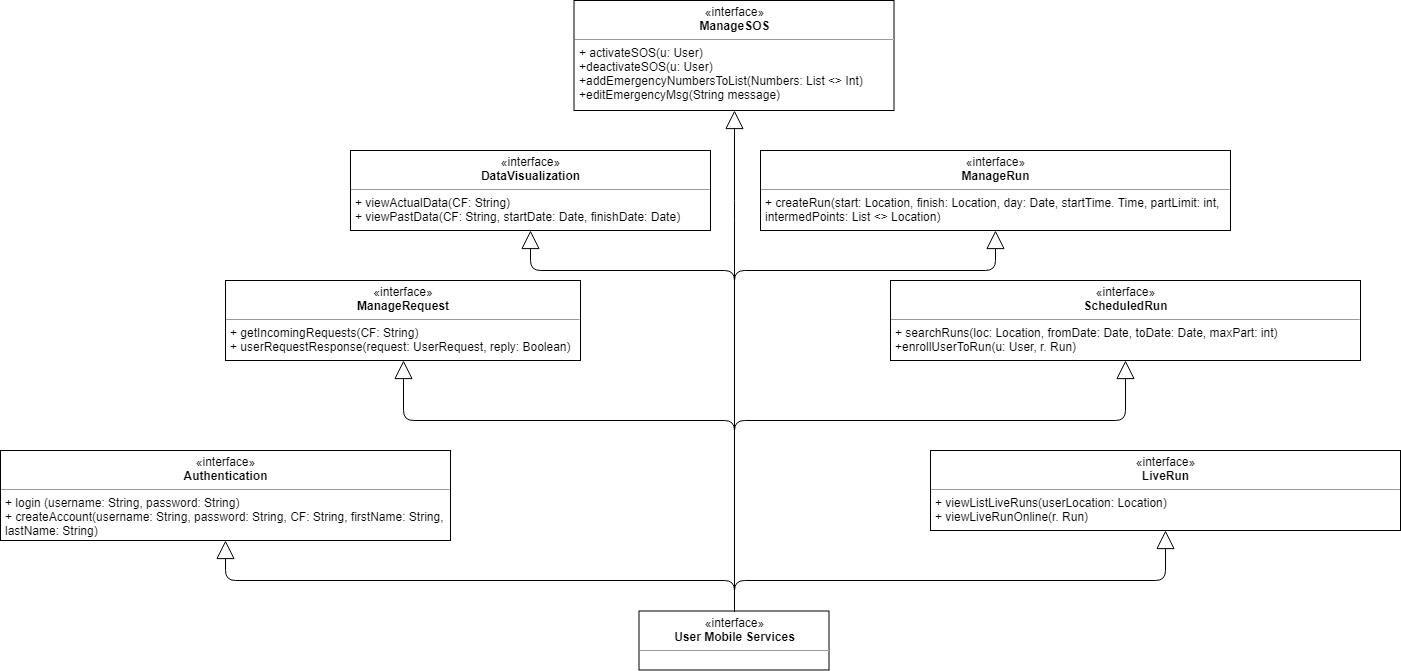
\includegraphics[scale=0.35]{./Pictures/compInterfDiagUserDD.png}
   
\end{figure}

\newpage